\section{Introduction}
\label{sec: introduction}
%
The basic setup of generative modelling involves using a dataset of observations of $\mathbf{x}$ to estimate the marginal distribution $p(\mathbf{x})$. Estimating $p(\mathbf{x})$ accurately enables various useful things such as: (i) sample generation; (ii) density estimation; (iii) compression; (iv) data imputation; (v) model selection, etc. Since $p(\mathbf{x})$ is unknown, we must approximate it with a model $p_{\boldsymbol{\theta}}(\mathbf{x}) \approx p(\mathbf{x})$, by optimizing some parameters $\boldsymbol{\theta}$. There are many ways to estimate $p(\mathbf{x})$; we focus on Variational Diffusion Models (VDMs)~\citep{kingma2021variational,kingma2023understanding}, which are a family of diffusion-based generative models~\citep{sohl2015deep}. Despite the growing popularity of diffusion models, gaining a deep understanding of the model class remains somewhat elusive for the uninitiated in non-equilibrium statistical physics. Hence, we present a more straightforward introduction to diffusion models using directed graphical modelling and variational inference principles, which imposes relatively fewer prerequisites on the average reader.

With that in mind, the goal of this paper is to provide a thorough introduction to VDMs, without overlooking mathematical details or introducing new notation relative to the seminal works. We start by reviewing the basic fundamental principles and motivations behind Variational Autoencoders (VAEs)~\citep{kingma2013auto,rezende2014stochastic}, and their hierarchical counterparts~\citep{salimans2015markov,sonderby2016ladder,kingma2016improved}. We then introduce diffusion probabilistic models as a natural extension of discrete-time hierarchical VAEs with a particular choice of inference and generative model, before delving into continuous-time variants which represent infinitely deep VAEs.

Variational perspectives on diffusion have also been studied by~\cite{tzen2019neural,huang2021variational,vahdat2021score}; we focus on VDMs since they represent the smoothest transition from VAEs to diffusion models. Our work is complementary to~\cite{luo2022understanding}, as they too provide an introduction to diffusion models. However, our exposition is far more comprehensive, up-to-date, and mathematically consistent with the seminal works on VDMs~\citep{kingma2021variational,kingma2023understanding}. Furthermore, we cover recent material on VDMs\texttt{++}~\citep{kingma2023understanding} and provide additional instructive insights which we hope will contribute to the dissemination and understanding of this model class.
%
\subsection{Variational Autoencoder}
%
Variational autoencoder models assume that data $\mathbf{x} \in \mathcal{X}^D$ are generated by some random process involving an unobserved random variable $\mathbf{z} \in \mathcal{Z}^K$. The marginal distribution of $\mathbf{x}$ is: $p(\mathbf{x}) = \int p(\mathbf{x}, \mathbf{z})\mathop{\mathrm{d}\mathbf{z}}$. 

The generative process is straightforward: (i) sample a latent variable from a prior distribution $\mathbf{z} \sim p(\mathbf{z})$; (ii) sample an observation from a conditional distribution $\mathbf{x}\sim p(\mathbf{x} \mid \mathbf{z})$. If we choose $\mathbf{z}$ to be a discrete random variable and $p(\mathbf{x} \mid \mathbf{z})$ to be a Gaussian distribution, then $p(\mathbf{x})$ is a Gaussian mixture. If we instead choose $\mathbf{z}$ to be a continuous random variable, then $p(\mathbf{x})$ represents an \textit{infinite} mixture of Gaussians.
% Judicious choices for the parametric form of these distributions depend on the data domain, e.g. Gaussian for continuous variables.

% Inference in Bayesian models amounts to computing the posterior over the latent variables $p(\mathbf{z} \mid \mathbf{x}) = p(\mathbf{x}, \mathbf{z}) / \int p(\mathbf{x}, \mathbf{z}) \mathop{\mathrm{d}\mathbf{z}}$. 
For complicated non-linear likelihood functions where $p(\mathbf{x} \mid \mathbf{z})$ is parameterized by a deep neural network, integrating out the latent variable $\mathbf{z}$ to compute $p(\mathbf{x})$ has no analytic solution, so we must rely on approximations. A straightforward Monte Carlo approximation of $p(\mathbf{x})$ is certainly possible: 
%
\begin{align}
&p(\mathbf{x}) = \mathbb{E}_{\mathbf{z} \sim p(\mathbf{z})} \left[p(\mathbf{x} \mid \mathbf{z})\right] \approx
\frac{1}{N}\sum_{i=1}^N p(\mathbf{x} \mid \mathbf{z}_i), &\mathbf{z}_1,\dots,\mathbf{z}_N \mathop{\sim}\limits^{\mathrm{iid}} p(\mathbf{z}), &
\end{align}
%
but is subject to the \textit{curse of dimensionality}, since the number of samples needed to properly cover the latent space grows exponentially with the dimensionality of the latent variable $\mathbf{z}$.

Alternatively, we can turn to variational methods, which pose probabilistic inference as an optimization problem~\citep{jordan1999introduction}. The first thing to note is that the intractability of $p(\mathbf{x})$ is related to the intractability of the true posterior over the latent variable $p(\mathbf{z} \mid \mathbf{x})$ through a basic identity:
%
\begin{align}
    &&p(\mathbf{x}) = \frac{p(\mathbf{x} \mid \mathbf{z})p(\mathbf{z})}{p(\mathbf{z} \mid \mathbf{x})},
    &&
    \mathrm{where}
    &&p(\mathbf{z} 
    \mid \mathbf{x}) = \frac{p(\mathbf{x} \mid \mathbf{z})p(\mathbf{z})}{\int p(\mathbf{x} \mid \mathbf{z})p(\mathbf{z})\mathop{\mathrm{d}\mathbf{z}}}.&&
\end{align}
%
Using a complicated neural network-based likelihood renders the integral on the RHS intractable. To estimate $p(\mathbf{x})$ we can approximate the true posterior $p(\mathbf{z} \mid \mathbf{x})$ via a parametric inference model $q(\mathbf{z} \mid \mathbf{x})$ of our choice, such that $q(\mathbf{z} \mid \mathbf{x}) \approx p(\mathbf{z} \mid \mathbf{x})$. Learning a single function with shared variational parameters $\boldsymbol{\phi}$ to map each datapoint $\mathbf{x}$ to a posterior distribution $q(\mathbf{z} \mid \mathbf{x})$ is known as \textit{amortized inference}. 
% Alternatively, optimizing distinct variational parameters for each individual datapoint $\mathbf{x}$ is equally valid, more expressive, but much less efficient, as it typically involves a per-datapoint optimization loop known as \textit{coordinate-ascent} variational inference.

We may optionally write $q_{\boldsymbol{\phi}}(\mathbf{z} \mid \mathbf{x})$ and $p_{\boldsymbol{\theta}}(\mathbf{x} \mid \mathbf{z})$ to explicitly state that these are parametric distributions realized by an encoder-decoder setup with variational parameters $\boldsymbol{\phi}$ and model parameters $\boldsymbol{\theta}$. The typical VAE setup specifies a prior $p(\mathbf{z})$ with no learnable parameters, and it is often chosen to be standard Gaussian: $p(\mathbf{z}) = \mathcal{N}(\mathbf{z}; 0, \mathbf{I})$. It is important to note that unlike the latent variable(s) $\mathbf{z}$ which are \textit{local}, the parameters $\{\boldsymbol{\phi}, \boldsymbol{\theta}\}$ are \textit{global} since they are shared for all datapoints. To improve our approximation, we'd like to minimize the Kullback-Leibler (KL) divergence $\argmin_{q(\mathbf{z} \mid \mathbf{x})} D_{\mathrm{KL}} \left(q(\mathbf{z} \mid \mathbf{x}) \parallel p(\mathbf{z} \mid \mathbf{x}) \right)$, but it is not possible do so directly as we do not have access to the true posterior $p(\mathbf{z} \mid \mathbf{x})$ for evaluation.

VAEs maximise the Variational Lower Bound (VLB) of $\log p(\mathbf{x})$:
%
\begin{align}
    D_{\mathrm{KL}} \left(q(\mathbf{z} \mid \mathbf{x}) \parallel p(\mathbf{z} \mid \mathbf{x}) \right) &=  \int q(\mathbf{z} \mid \mathbf{x})  \log \frac{q(\mathbf{z} \mid \mathbf{x})}{p(\mathbf{z} \mid \mathbf{x})} \mathop{\mathrm{d}\mathbf{z}} 
    \\[5pt] &= \mathbb{E}_{q(\mathbf{z} \mid \mathbf{x})} \left[  \log q(\mathbf{z} \mid \mathbf{x}) - \log \frac{p(\mathbf{x}, \mathbf{z})}{p(\mathbf{x})}\right]
    \\[5pt] &= \mathbb{E}_{q(\mathbf{z} \mid \mathbf{x})} \left[  \log q(\mathbf{z} \mid \mathbf{x}) - \log p(\mathbf{x}, \mathbf{z}) \right] + \log p(\mathbf{x})
    \\[5pt] &= -\mathrm{VLB}(\mathbf{x}) + \log p(\mathbf{x}),
\end{align}
%
adding $\mathrm{VLB}(\mathbf{x})$ to both sides reveals:
%
\begin{align}
    D_{\mathrm{KL}} \left(q(\mathbf{z} \mid \mathbf{x}) \parallel p(\mathbf{z} \mid \mathbf{x}) \right) + \mathrm{VLB}(\mathbf{x}) = \log p(\mathbf{x}) \implies \log p(\mathbf{x}) \geq \mathrm{VLB}(\mathbf{x}),
\end{align}
as $D_{\mathrm{KL}} \left(q(\mathbf{z} \mid \mathbf{x}) \parallel p(\mathbf{z} \mid \mathbf{x}) \right) \geq 0$ by Gibbs' inequality. Hence, maximizing the VLB implicitly minimizes the KL divergence of $q(\mathbf{z} \mid \mathbf{x})$ from the true posterior $p(\mathbf{z} \mid \mathbf{x})$ as desired. The VLB is also known as the Evidence Lower BOund (ELBO) since $p(\mathbf{x})$ is called the \textit{evidence}. The VLB optimized by VAEs is:
%
\begin{align}
    \mathrm{VLB}(\mathbf{x}) &= \mathbb{E}_{q(\mathbf{z} \mid \mathbf{x})} \left[\log \frac{p(\mathbf{x}, \mathbf{z})}{q(\mathbf{z} \mid \mathbf{x})}\right]
    \\[5pt] &= \mathbb{E}_{q(\mathbf{z} \mid \mathbf{x})} \left[\log p(\mathbf{x} \mid \mathbf{z})\right]
    + \mathbb{E}_{q(\mathbf{z} \mid \mathbf{x})} \left[\log \frac{p(\mathbf{z})}{q(\mathbf{z} \mid \mathbf{x})} \right]
    \\[5pt] &= \mathbb{E}_{q(\mathbf{z} \mid \mathbf{x})} \left[\log p(\mathbf{x} \mid \mathbf{z})\right] - D_{\mathrm{KL}} \left(q(\mathbf{z} \mid \mathbf{x}) \parallel p(\mathbf{z}) \right),
\end{align}
%
which amounts to an expected likelihood objective regularized by the KL of the posterior from the prior.
% Optimizing this objective amounts to maximizing the expected likelihood $p(\mathbf{x} \mid \mathbf{z})$ of observing $\mathbf{x}$ under our approximate posterior $q(\mathbf{z} \mid \mathbf{x})$, regularized by the KL divergence of $q(\mathbf{z} \mid \mathbf{x})$ from the prior $p(\mathbf{z})$. 
If we let $\mathcal{D}$ be a dataset of i.i.d. data, then $\mathrm{VLB}(\mathcal{D}) = \sum_{\mathbf{x} \in \mathcal{D}}\mathrm{VLB}(\mathbf{x})$. We can use stochastic variational inference~\citep{hoffman2013stochastic} and the \textit{reparameterization trick}~\citep{kingma2013auto,rezende2014stochastic} to \textit{jointly} optimize the VLB w.r.t. the model parameters $\boldsymbol{\theta}$, and variational parameters $\boldsymbol{\phi}$. For more details on this procedure, the reader may refer to~\cite{kingma2019introduction} and \cite{blei2017variational}.
%

\begin{figure}[!t]
    \centering
    \hfill
    \begin{subfigure}{.32\columnwidth}
        \centering       
        \begin{tikzpicture}[thick,scale=1, every node/.style={scale=1}]
            \node[latent] (zt) {$\mathbf{z}_T$};
            \draw node[draw=none, scale=0.75, below=6pt of zt] (z3) {\hspace{0.5pt}\rotatebox{90}{$\mathbf{\cdots}$}};
            \node[latent, below=13pt of z3] (z2) {$\mathbf{z}_2$};
            \node[latent, below=15pt of z2] (z1) {$\mathbf{z}_1$};
            \node[obs, below=15pt of z1] (x) {$\mathbf{x}$};
            \edge[-]{zt}{z3}
            \edge[-{Latex[scale=1.0]}]{z3}{z2}
            \edge[-{Latex[scale=1.0]}]{z2}{z1}
            \edge[-{Latex[scale=1.0]}]{z1}{x}
            \node[latent, draw=none, right=-2pt of z2, yshift=-16pt] (eq2) {$p(\mathbf{z}_1 \mid \mathbf{z}_2)$};
            \node[latent, draw=none, right=-2pt of z1, yshift=-16pt] (eq1) {$p(\mathbf{x} \mid \mathbf{z}_1)$};
            \node[latent, draw=none, right=-2pt of z3, xshift=6pt, yshift=-0pt] (eq3) {$p(\mathbf{z}_{t-1} \mid \mathbf{z}_t)$};
        \end{tikzpicture}
        \caption{Hierarchical Generative Model}
    \end{subfigure}
    \hfill
    \begin{subfigure}{.32\columnwidth}
        \centering
        \begin{tikzpicture}[thick,scale=1, every node/.style={scale=1}]
            \node[latent] (zt) {$\mathbf{z}_T$};
            \draw node[draw=none, scale=0.75, below=13pt of zt] (z3) {\hspace{0.5pt}\rotatebox{90}{$\mathbf{\cdots}$}};
            \node[latent, below=6pt of z3] (z2) {$\mathbf{z}_2$};
            \node[latent, below=15pt of z2] (z1) {$\mathbf{z}_1$};
            \node[obs, below=15pt of z1] (x) {$\mathbf{x}$};
            \edge[-{Latex[scale=1.0]}]{z3}{zt}
            \edge[-]{z2}{z3}
            \edge[-{Latex[scale=1.0]}]{z1}{z2}
            \edge[-{Latex[scale=1.0]}]{x}{z1}
            \node[latent, draw=none, right=-2pt of z2, yshift=-16pt] (eq2) {$q(\mathbf{z}_2 \mid \mathbf{z}_1)$};
            \node[latent, draw=none, right=-2pt of z1, yshift=-16pt] (eq1) {$q(\mathbf{z}_1 \mid \mathbf{x})$};
            \node[latent, draw=none, right=-2pt of z3, xshift=6pt, yshift=-0pt] (eq3) {$q(\mathbf{z}_{t} \mid \mathbf{z}_{t-1})$};
        \end{tikzpicture}
        \caption{Bottom-up Inference Model}
    \end{subfigure}
    \hfill
    \begin{subfigure}{.32\columnwidth}
        \centering
        \begin{tikzpicture}[thick,scale=1, every node/.style={scale=1}]
            \node[obs] (x) {$\mathbf{x}$};
            \node[latent, below=15pt of x] (zt) {$\mathbf{z}_T$};
            \draw node[draw=none, scale=0.75, below=6pt of zt] (z3) {\hspace{0.5pt}\rotatebox{90}{$\mathbf{\cdots}$}};
            \node[latent, below=13pt of z3] (z2) {$\mathbf{z}_2$};
            \node[latent, below=15pt of z2] (z1) {$\mathbf{z}_1$};
            \edge[-{Latex[scale=1.0]}]{x}{zt}
            \edge[-]{zt}{z3}
            \edge[-{Latex[scale=1.0]}]{z3}{z2}
            \edge[-{Latex[scale=1.0]}]{z2}{z1}
            \draw [-{Latex[scale=1.0]}] (x) to [out=225,in=135] (z2);
            \draw [-{Latex[scale=1.0]}] (x) to [out=225,in=135] (z1);
            \node[latent, draw=none, right=-2pt of x, yshift=-16pt] (eq1) {$q(\mathbf{z}_T \mid \mathbf{x})$};
            \node[latent, draw=none, right=-2pt of z2, yshift=-16pt] (eq2) {$q(\mathbf{z}_1 \mid \mathbf{z}_2, \mathbf{x})$};
            \node[latent, draw=none, right=-2pt of z3, xshift=6pt, yshift=-0pt] (eq3) {$q(\mathbf{z}_{t-1} \mid \mathbf{z}_{t}, \mathbf{x})$};
        \end{tikzpicture}
        \caption{Top-down Inference Model}
    \end{subfigure}
    \hfill
    \caption{Hierarchical latent variable graphical models. (a) The generative model $p(\mathbf{x}, \mathbf{z}_{1:T})$ of a hierarchical VAE with $T$ latent variables is a Markov chain. (b) The standard \textit{bottom-up} inference model $q(\mathbf{z}_{1:T} \mid \mathbf{x})$ of a hierarchical VAE is a Markov chain in the reverse direction. (c) The \textit{top-down} inference model follows the same topological ordering of the latent variables as the generative model. This top-down structure is used to specify diffusion models. In diffusion models the posterior $q(\mathbf{z}_{1:T} \mid \mathbf{x})$ is tractable due to Gaussian conjugacy, which enables us to specify the \textit{generative} model transitions as $p(\mathbf{z}_{t-1} \mid \mathbf{z}_{t}) = q(\mathbf{z}_{t-1} \mid \mathbf{z}_{t}, \mathbf{x} = \hat{\mathbf{x}}_{\boldsymbol{\theta}}(\mathbf{z}_t; t))$,  where the data $\mathbf{x}$ is replaced by a denoising model $\hat{\mathbf{x}}_{\boldsymbol{\theta}}(\mathbf{z}_t; t)$.
    }
    \label{fig: hvae}
\end{figure}

\subsection{Hierarchical VAE}
\label{subsec: Hierarchical VAE}
A hierarchical VAE is a deep latent variable model comprised of a hierarchy of latent variables $\mathbf{z}_1,\mathbf{z}_2 \dots, \mathbf{z}_T$. Introducing additional (auxiliary) latent variables significantly improves the flexibility of both inference and generative models~\citep{salimans2015markov,ranganath2016hierarchical,maaloe2016auxiliary}.

The joint distribution $p(\mathbf{x}, \mathbf{z}_{1:T})$ specifying a generative model of $\mathbf{x}$ is a variational Markov chain \newline $\mathbf{z}_T \to \mathbf{z}_{T-1} \to \cdots \to \mathbf{z}_1 \to \mathbf{x}$:
%
\begin{align}
    p(\mathbf{x}, \mathbf{z}_{1:T}) &= p(\mathbf{z}_T)p(\mathbf{z}_{T-1} \mid \mathbf{z}_T) \cdots p(\mathbf{z}_1 \mid \mathbf{z}_2) p(\mathbf{x} \mid \mathbf{z}_1)
    \\[5pt] & 
    = p(\mathbf{z}_T) \left[\prod_{t=2}^{T}p(\mathbf{z}_{t-1} \mid \mathbf{z}_t)\right]p(\mathbf{x} \mid \mathbf{z}_1). \label{eq: hvae_gen}
\end{align}
%
The approximate posterior $q(\mathbf{z}_{1:T} \mid \mathbf{x})$ is a Markov chain in the reverse (bottom-up) direction \newline $\mathbf{z}_T \leftarrow \mathbf{z}_{T-1} \leftarrow \cdots \leftarrow \mathbf{z}_1 \leftarrow \mathbf{x}$:
%
\begin{align}
    q(\mathbf{z}_{1:T} \mid \mathbf{x}) &= q(\mathbf{z}_1 \mid \mathbf{x})q(\mathbf{z}_2 \mid \mathbf{z}_1)q(\mathbf{z}_3 \mid \mathbf{z}_2) \cdots q(\mathbf{z}_T \mid \mathbf{z}_{T-1})
    \\[5pt] & 
    = q(\mathbf{z}_1 \mid \mathbf{x}) \prod_{t=2}^{T}q(\mathbf{z}_{t} \mid \mathbf{z}_{t-1}). \label{eq: hvae_inf}
\end{align}
%
The marginal likelihood $p(\mathbf{x})$ is obtained by marginalizing out the latent variables:
%
\begin{align}
    && p(\mathbf{x}) 
    = \int p(\mathbf{x} \mid  \mathbf{z}_{1})p(\mathbf{z}_1) \mathop{\mathrm{d}\mathbf{z}_{1}},
    &&
    % \mathrm{where}&&
    p(\mathbf{z}_t) 
    = \int p(\mathbf{z}_t \mid  \mathbf{z}_{t+1})p(\mathbf{z}_{t+1}) \mathop{\mathrm{d}\mathbf{z}_{t+1}},&&t = 1,2,\dots,T-1,&&
\end{align}
%
and the model is fit by maximizing the VLB of $\log p(\mathbf{x})$:
%
\begin{align}
    \log p(\mathbf{x}) \geq \mathbb{E}_{q(\mathbf{z}_{1:T} \mid \mathbf{x})} \left[ \log \frac{p(\mathbf{x}, \mathbf{z}_{1:T})}{q(\mathbf{z}_{1:T} \mid \mathbf{x})} \right] \eqqcolon \mathrm{VLB}(\mathbf{x}).
\end{align}
%
\subsection{Generative Feedback}
\label{subsec: Generative Feedback}
%
\begin{wrapfigure}[21]{r}{0.4\textwidth}
    \centering
    \vspace{-28pt}
    \begin{tikzpicture}[thick,scale=1, every node/.style={scale=1}]
        \node[latent] (zt) {$\hat{\mathbf{z}}_T$};
        \draw node[draw=none, scale=0.75, below=6pt of zt] (z3) {\hspace{0.5pt}\rotatebox{90}{$\mathbf{\cdots}$}};
        \node[latent, below=13pt of z3] (z2) {$\hat{\mathbf{z}}_2$};
        \node[latent, below=15pt of z2] (z1) {$\hat{\mathbf{z}}_1$};
        \edge[-]{zt}{z3}
        \edge[-{Latex[scale=1.0]}]{z3}{z2}
        \edge[-{Latex[scale=1.0]}]{z2}{z1}

        \node[latent, left=25pt of zt] (zzt) {$\mathbf{z}_T$};
        \draw node[draw=none, scale=0.75, below=13pt of zzt] (zz3) {\hspace{0.5pt}\rotatebox{90}{$\mathbf{\cdots}$}};
        \node[latent, left=25pt of z2] (zz2) {$\mathbf{z}_2$};
        \node[latent, left=25pt of z1] (zz1) {$\mathbf{z}_1$};
        \node[obs, below=15pt of zz1] (xx) {$\mathbf{x}$};

        \node[latent, draw=none, left=15pt of zzt] (st) {$\mathcal{N}(0,\sigma_T^2)$};
        \edge[-{Latex[scale=1.0]}]{st}{zzt}
        \node[latent, draw=none, left=15pt of zz2] (s2) {$\mathcal{N}(0,\sigma_2^2)$};
        \edge[-{Latex[scale=1.0]}]{s2}{zz2}
        \node[latent, draw=none, left=15pt of zz1] (s1) {$\mathcal{N}(0,\sigma_1^2)$};
        \edge[-{Latex[scale=1.0]}]{s1}{zz1}

        \node[latent, draw=none, right=25pt of zt] (dt) {$\mathbf{d}_T$};
        \draw node[draw=none, scale=0.75, below=13pt of dt] (d3) {\hspace{0.5pt}\rotatebox{90}{$\mathbf{\cdots}$}};
        \node[latent, draw=none, right=25pt of z2] (d2) {$\mathbf{d}_2$};
        \node[latent, draw=none, right=25pt of z1] (d1) {$\mathbf{d}_1$};
        \node[obs, below=15pt of d1] (x) {$\mathbf{x}$};
        
        \edge[blue, -{Latex[scale=1.0]}]{d3}{dt}
        \edge[blue, -]{d2}{d3}
        \edge[blue, -{Latex[scale=1.0]}]{d1}{d2}
        \edge[blue, -{Latex[scale=1.0]}]{x}{d1}
        \edge[densely dashed,-]{dt}{zt}
        \edge[densely dashed,-]{d2}{z2}
        \edge[densely dashed,-]{d1}{z1}
        \edge[blue,-{Latex[scale=1.0]}]{xx}{zz1}
        \edge[blue,-{Latex[scale=1.0]}]{zz1}{zz2}
        \edge[blue,-]{zz2}{zz3}
        \edge[blue,-{Latex[scale=1.0]}]{zz3}{zzt}
        \edge[-{Latex[scale=1.0]}]{zzt}{zt}
        \edge[-{Latex[scale=1.0]}]{zz2}{z2}
        \edge[-{Latex[scale=1.0]}]{zz1}{z1}
    \end{tikzpicture}
    \caption{A Ladder Network. The latent variables $\mathbf{z}_1, \mathbf{z}_2, \dots, \mathbf{z}_T$ are noisy representations of $\mathbf{x}$, and $\mathbf{d}_1, \mathbf{d}_2, \dots, \mathbf{d}_T$ are clean representations; both sets are produced by a shared encoder (blue arrows). The variables $\hat{\mathbf{z}}_1, \hat{\mathbf{z}}_2, \dots, \hat{\mathbf{z}}_T$ are outputs of denoising functions where $\hat{\mathbf{z}}_t = g_t(\mathbf{z}_t, \hat{\mathbf{z}}_{t+1})$. Notice how $g_t(\cdot)$ receives both bottom-up and top-down information. The dashed horizontal lines denote local cost functions used to minimize  $\|\hat{\mathbf{z}}_t - \mathbf{d}_t \|^2_2$. The main difference compared to denoising diffusion models is that here the denoising targets $\mathbf{d}_t$ are learned representations of $\mathbf{x}$.
    }
    \label{fig: ladder}
\end{wrapfigure}
%
The trouble with hierarchical latent variable models with bottom-up inference is bottom-up inference.~\cite{burda2015importance} and~\cite{sonderby2016ladder} both found hierarchical models with purely bottom-up inference are typically not capable of utilizing more than two layers of latent variables. This often manifests as \textit{posterior collapse}, whereby the posterior distribution (of the top-most layer, say) collapses to a standard Gaussian prior, failing to learn meaningful representations and effectively deactivating latent variables.

To understand why bottom-up inference is challenging for even modestly deep hierarchies, we start by noting the asymmetry between the associated generative and inference models in Equations~\ref{eq: hvae_gen} and~\ref{eq: hvae_inf} respectively.~\cite{burda2015importance,sohl2015deep} point this out as a source of difficulty in training the inference model efficiently, since there is no way to express each term in the VLB as an expectation under a distribution over a single latent variable.~\cite{luo2022understanding} present a similar efficiency-based argument against using bottom-up inference in hierarchical latent variable models.

We claim that efficiency arguments paint an incomplete picture; the main reason one should avoid bottom-up inference is the lack of direct \textit{feedback} from the generative model.
To show why generative feedback is important, we stress that the purpose of the inference model is to perform \textit{Bayesian inference} at any given layer in the hierarchy. That is, to compute the posterior distribution $q(\mathbf{z}_t \mid \mathbf{x})$ over each latent variable $\mathbf{z}_t$:
%
\begin{align}
    & q(\mathbf{z}_t \mid \mathbf{x}) = \frac{p(\mathbf{x} \mid \mathbf{z}_t)p(\mathbf{z}_t)}{p(\mathbf{x})}
    \propto p(\mathbf{x} \mid \mathbf{z}_t) \int p(\mathbf{z}_t \mid  \mathbf{z}_{t+1})p(\mathbf{z}_{t+1}) \mathop{\mathrm{d}\mathbf{z}_{t+1}}, \label{eq: qzx_bayes}
\end{align}
%
which clearly shows that the posterior is not only proportional to the current layer's prior $p(\mathbf{z}_t)$ but also to the layer above's $p(\mathbf{z}_{t+1})$, and so on, following the reverse of the generative Markov chain (Equation~\ref{eq: hvae_gen}). 

It therefore stands to reason that interleaving feedback from each transition in the generative model into each respective transition in the inference model can only make the inference network more accurate. To that end, we can take Equation~\ref{eq: qzx_bayes} and rewrite the posterior distribution over each $\mathbf{z}_t$ such that it contains a more explicit dependency on the preceding latent variables as prescribed:
%
\begin{align}
    & q(\mathbf{z}_t \mid \mathbf{x}) = \int q(\mathbf{z}_t \mid \mathbf{z}_{t+1}, \mathbf{x}) \mathop{\mathrm{d}\mathbf{z}_{t+1}} 
    % \\[5pt] & 
    \propto \int p(\mathbf{x} \mid \mathbf{z}_t) p(\mathbf{z}_t \mid  \mathbf{z}_{t+1})p(\mathbf{z}_{t+1})\mathop{\mathrm{d}\mathbf{z}_{t+1}}
    \\[5pt] \implies \ & q(\mathbf{z}_{t-1} \mid \mathbf{z}_{t}, \mathbf{x}) \propto p(\mathbf{x} \mid \mathbf{z}_{t-1}) p(\mathbf{z}_{t-1} \mid  \mathbf{z}_{t})p(\mathbf{z}_{t}).
\end{align}
%
The posterior $q(\mathbf{z}_{t-1} \mid \mathbf{z}_{t}, \mathbf{x})$ now follows the same topological ordering of the latent variables as the prior $p(\mathbf{z}_{t-1} \mid \mathbf{z}_t)$, and it coincides with the \textit{top-down} inference model in HVAEs~\citep{sonderby2016ladder,kingma2016improved}. Figure~\ref{fig: hvae} shows how this top-down structure compares to the bottom-up approach. An added benefit of the top-down approach is that the generative model can also receive data-dependent feedback from the inference procedure, which~\cite{sonderby2016ladder} found to be beneficial in practice. 

\cite{valpola2015neural,rasmus2015semi} were the first to introduce such lateral feedback connections between the inference and generative paths in hierarchical latent variable models. They called their denoising autoencoder a \textit{ladder network} (see Figure~\ref{fig: ladder}), which later inspired the ladder VAE~\citep{sonderby2016ladder}.~\cite{valpola2015neural} argue that incorporating lateral feedback connections enables the higher layers to learn abstract invariant representations as they no longer have to retain all the details about the input. Concretely, as depicted in Figure~\ref{fig: ladder}, each denoised variable $\hat{\mathbf{z}}_t \coloneqq g_t(\mathbf{z}_t, \hat{\mathbf{z}}_{t+1})$ is computed using a denoising function $g_t(\cdot)$ which receives bottom-up feedback from $\mathbf{z}_t$ and top-down feedback from $\hat{\mathbf{z}}_{t+1}$.
%
\subsection{Top-down Inference}
\label{subsec: Top-down Inference Model}
%
The joint approximate posterior $q(\mathbf{z}_{1:T} \mid \mathbf{x})$ can be alternatively factorized into the \textit{top-down} inference model~\citep{sonderby2016ladder,kingma2016improved}. As mentioned in Section~\ref{subsec: Generative Feedback}, the top-down inference model follows the same topological ordering of the latent variables as the generative model, that is:
%
\begin{align}
    q(\mathbf{z}_{1:T} \mid \mathbf{x}) & = q(\mathbf{z}_T \mid \mathbf{x}) q(\mathbf{z}_{T-1} \mid \mathbf{z}_{T}, \mathbf{x}) \cdots q(\mathbf{z}_2 \mid \mathbf{z}_3, \mathbf{x})q(\mathbf{z}_1 \mid \mathbf{z}_2, \mathbf{x})
    \\[5pt] & 
    = q(\mathbf{z}_T \mid \mathbf{x}) \prod_{t=2}^{T} q(\mathbf{z}_{t-1} \mid \mathbf{z}_t, \mathbf{x}).
\end{align}
%
Variants of the top-down inference model have featured in much deeper state-of-the-art HVAEs for sample generation~\citep{maaloe2019biva,vahdat2020nvae,child2020very,shu2022bit} and approximate counterfactual inference~\citep{pmlr-v202-de-sousa-ribeiro23a,monteiro2022measuring}. As we will explain later, the top-down hierarchical latent variable model serves as the basis for parameterizing denoising diffusion models~\citep{sohl2015deep,ho2020denoising,kingma2021variational}. 

For now, we derive the corresponding VLB to obtain a concrete optimization objective:
%
\begin{align}
    \mathrm{VLB}(\mathbf{x}) & = \mathbb{E}_{q(\mathbf{z}_{1:T} \mid \mathbf{x})} \left[ \log \frac{p(\mathbf{x}, \mathbf{z}_{1:T})}{q(\mathbf{z}_{1:T} \mid \mathbf{x})} \right]
    \\[5pt] & = \mathbb{E}_{q(\mathbf{z}_{1:T} \mid \mathbf{x})} \left[ \log \frac{p(\mathbf{z}_T) p(\mathbf{x} \mid \mathbf{z}_1) \prod_{t=2}^{T}p(\mathbf{z}_{t-1} \mid \mathbf{z}_t)}{q(\mathbf{z}_T \mid \mathbf{x}) \prod_{t=2}^{T} q(\mathbf{z}_{t-1} \mid \mathbf{z}_t, \mathbf{x})} \right] \customtag{factor the joint}
    \\[5pt] & = \mathbb{E}_{q(\mathbf{z}_{1:T} \mid \mathbf{x})}\left[\log p(\mathbf{x} \mid \mathbf{z}_{1}) + \log \frac{p(\mathbf{z}_T)}{ q(\mathbf{z}_T \mid \mathbf{x})}\right] + \mathbb{E}_{q(\mathbf{z}_{1:T} \mid \mathbf{x})}\left[\sum_{t=2}^T \log  \frac{p(\mathbf{z}_{t-1} \mid \mathbf{z}_t)}{q(\mathbf{z}_{t-1} \mid \mathbf{z}_t, \mathbf{x})} \right]
    \\[5pt] & = \mathbb{E}_{q(\mathbf{z}_{1} \mid  \mathbf{x})}\left[\log p(\mathbf{x} \mid \mathbf{z}_{1})\right] + \mathbb{E}_{q(\mathbf{z}_{T} \mid \mathbf{x})}\left[\log \frac{p(\mathbf{z}_T)}{ q(\mathbf{z}_T \mid \mathbf{x})}\right] \nonumber \\[2pt] & \qquad\qquad\qquad\qquad\qquad\qquad\qquad + \sum_{t=2}^T \mathbb{E}_{q(\mathbf{z}_{t-1}, \mathbf{z}_{t} \mid \mathbf{x})} \left[\log \frac{p(\mathbf{z}_{t-1} \mid \mathbf{z}_t)}{q(\mathbf{z}_{t-1} \mid \mathbf{z}_t, \mathbf{x})} \right]
    \\[5pt] & = \mathbb{E}_{q(\mathbf{z}_{1} \mid  \mathbf{x})}\left[\log p(\mathbf{x} \mid \mathbf{z}_{1})\right] + \mathbb{E}_{q(\mathbf{z}_{T} \mid \mathbf{x})}\left[\log \frac{p(\mathbf{z}_T)}{ q(\mathbf{z}_T \mid \mathbf{x})}\right] \nonumber \\[2pt] & \qquad\qquad\qquad\qquad\qquad\qquad\qquad + \sum_{t=2}^T \mathbb{E}_{q(\mathbf{z}_{t} \mid \mathbf{x})} \left[\mathbb{E}_{q(\mathbf{z}_{t-1} \mid \mathbf{z}_{t}, \mathbf{x})} \left[ \log \frac{p(\mathbf{z}_{t-1} \mid \mathbf{z}_t)}{q(\mathbf{z}_{t-1} \mid \mathbf{z}_t, \mathbf{x})} \right]\right]
    \\[5pt] & = \mathbb{E}_{q(\mathbf{z}_{1} \mid \mathbf{x})}\left[\log p(\mathbf{x} \mid \mathbf{z}_{1})\right] - D_{\mathrm{KL}}(q(\mathbf{z}_{T} \mid \mathbf{x}) \parallel p(\mathbf{z}_{T})) \nonumber \\[2pt] & \qquad\qquad\qquad\qquad\qquad\qquad\qquad - \sum_{t=2}^T \mathbb{E}_{q(\mathbf{z}_{t} \mid \mathbf{x})} \left[D_{\mathrm{KL}}(q(\mathbf{z}_{t-1} \mid \mathbf{z}_{t}, \mathbf{x}) \parallel p(\mathbf{z}_{t-1} \mid \mathbf{z}_{t}))\right]. \label{eq: hvae_elbo}
\end{align}
%
It is well worth dedicating some time to understanding the details of the above derivation and the resulting expression, as it is the \textit{exact} objective optimized by diffusion models as well.

One thing to notice is that it comprises the familiar trade-off between minimizing input reconstruction error and keeping the (hierarchical) approximate posterior $q(\mathbf{z}_{1:T} \mid \mathbf{x})$ close to the prior $p(\mathbf{z}_{1:T})$. In contrast to standard VAEs, the prior in HVAEs is learned from data rather than being fixed, as this affords greater flexibility~\citep{kingma2016improved,hoffman2016elbo,tomczak2018vae}.

%
\begin{figure}
    \centering
    \begin{subfigure}{\columnwidth}
    \centering  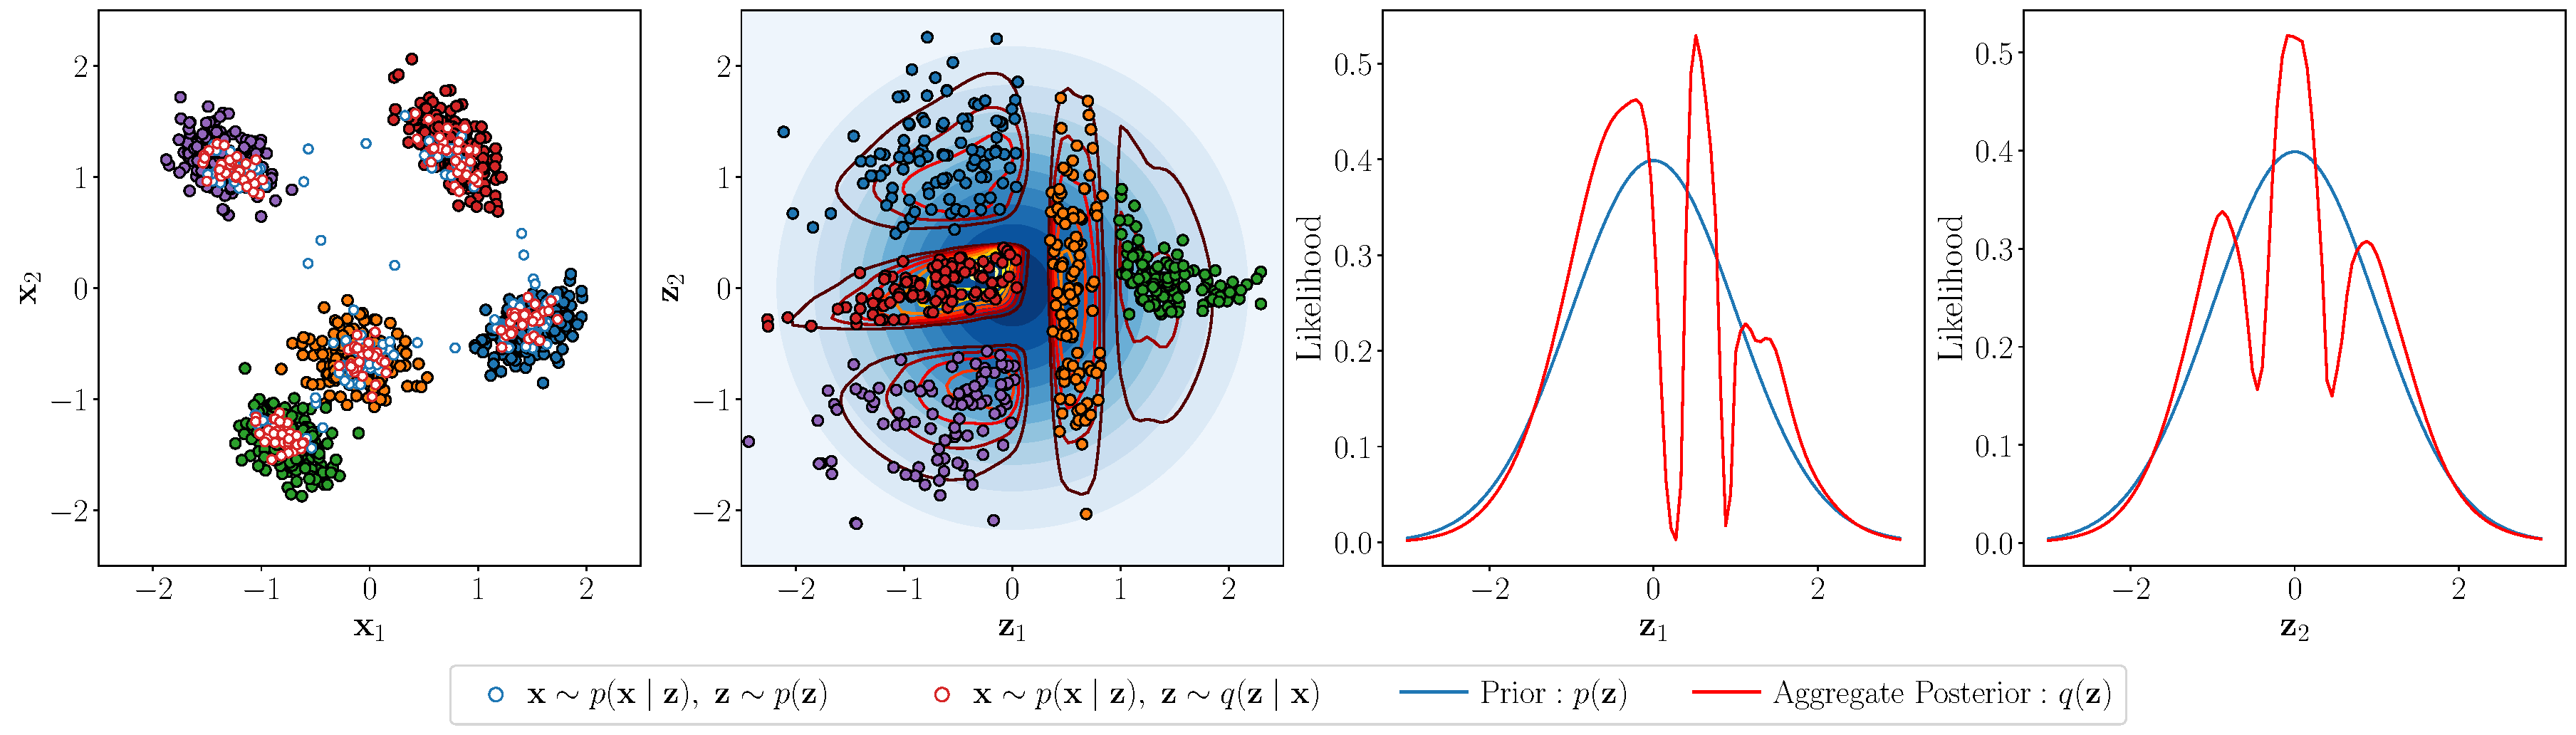
\includegraphics[trim=0 50 0 0, clip, width=\textwidth]{figures/hole2.pdf}
    \end{subfigure}
    \begin{subfigure}{\columnwidth}
    \centering    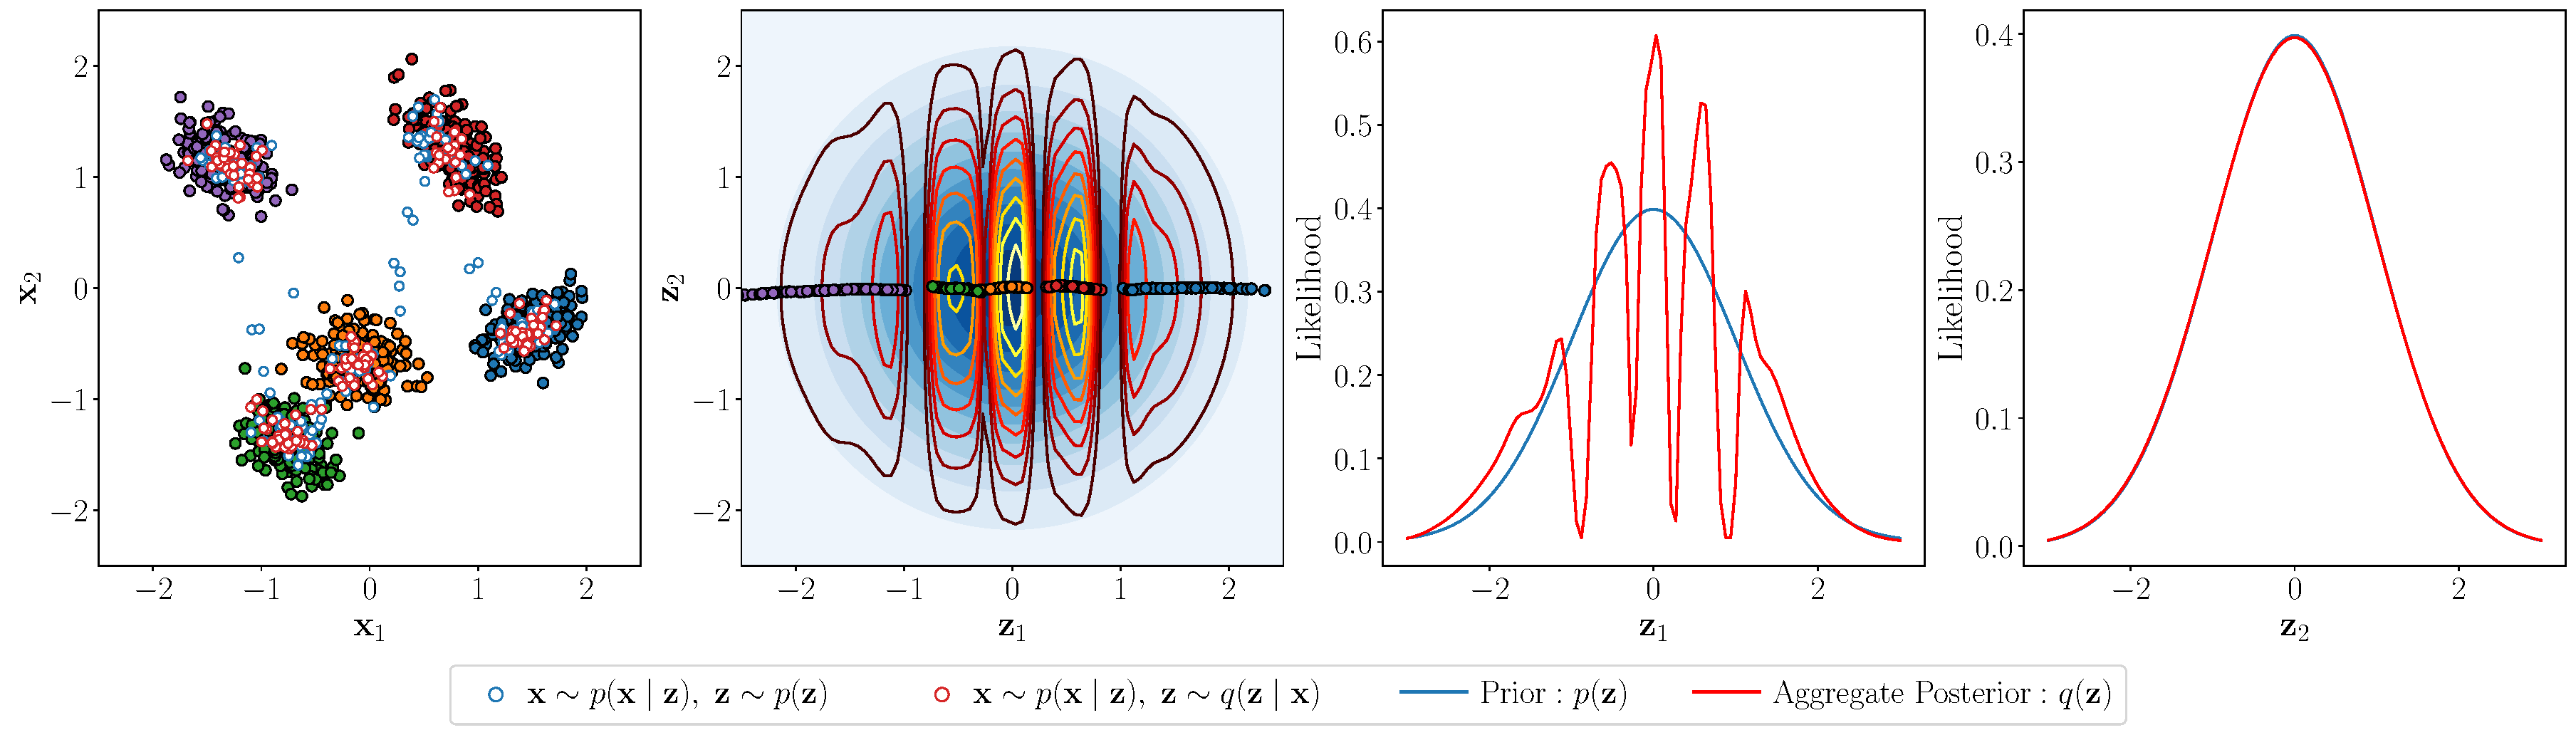
\includegraphics[width=\textwidth]{figures/hole.pdf}
    \end{subfigure}
    \caption{Demonstration of the \textit{hole problem} in VAEs. Results are from a single stochastic layer VAE trained on a 2D toy dataset with five clusters. The latent variable $\mathbf{z}$ is also 2-dimensional for illustration purposes.
    The leftmost column shows the dataset, overlaid with reconstructed datapoints (red border) and random samples from the generative model (blue border). The remaining columns show the assumed prior $p(\mathbf{z}) = \mathcal{N}(\mathbf{z};0, \mathbf{I})$ (blue contours) overlaid with the aggregate posterior $q(\mathbf{z}) = \sum_{i=1}^N q(\mathbf{z} \mid \mathbf{x}_i) / N$. As shown, there are regions with high density under the prior which are assigned low density under the aggregate posterior. This affects the quality of the random samples since we are likely to sample from regions in $p(\mathbf{z})$ not covered by the data. Further, the bottom row shows a common occurrence in VAEs where latent variable(s) are not activated/used at all by the model, in this case, $\mathbf{z}_2$ was not used.
    }
    \label{fig: hole}
\end{figure}
%
\paragraph{The Problem with VAEs.}
%
A primary issue with VAEs is the \textit{hole problem}~\citep{rezende2018taming}. The hole problem refers to the mismatch between the so-called aggregate posterior $q(\mathbf{z})$ and the prior $p(\mathbf{z})$ over the latent variables~\citep{makhzani2015adversarial,hoffman2016elbo}. The aggregate posterior is simply the average posterior distribution over the dataset $\mathcal{D} = \{\mathbf{x}_i\}_{i=1}^N$, that is:
%
\begin{align}
    &&q(\mathbf{z}) = \int q(\mathbf{z} \mid \mathbf{x})p_\mathcal{D}(\mathbf{x}) \mathop{\mathrm{d}\mathbf{x}} 
    , && p_{\mathcal{D}}(\mathbf{x}) = \frac{1}{N}\sum_{i=1}^N \delta(\mathbf{x} - \mathbf{x}_i),&&
\end{align}
%
where $p_\mathcal{D}(\mathbf{x})$ is the \textit{empirical distribution}, constructed by a Dirac delta function $\delta(\cdot)$ centered on each training datapoint $\mathbf{x}_i$. As shown in Figure~\ref{fig: hole}, there can be regions with \textit{high} probability density under the prior which have \textit{low} density under the aggregate posterior. This affects the quality of generated samples when the decoder receives $\mathbf{z}$'s sampled from regions not covered by the data. As we will show, diffusion models circumvent this by defining the aggregate posterior to be equal to the prior by construction.